

\chapter{Planificación}

\section{Planificación temporal}

\subsection{Fases del proyecto}

En este apartado se mencionan cada una de las fases en las que se ha dividido el desarrollo del proyecto. Con cada fase se incluye una explicación de los temas desarrollados. En el siguiente apartado de la sección se encuentra el \textit{diagrama de Gantt} correspondiente.

\subsubsection{Fase inicial o de investigación}

En cuanto a la primera fase del desarrollo del proyecto, se comenzó con una investigación teórica sobre lo que es el trading, trading algorítmico y demás conceptos de economía que entran en juego en el tema. Aquí se realizó también una investigación sobre dos de los principales referentes del análisis de mercados: \textit{Charles Dow} y \textit{Richard Wyckoff}. \newline

En esta fase también se hicieron programas de ejemplo usando las distintas \textit{APIs} de conocidas plataformas de trading como son \textit{MetaTrader} o \textit{Binance} (específica para criptomonedas). \newline

Durante este período también se estuvo estudiando las posibles herramientas a usar para el proyecto. Se siguieron tutoriales de \textit{Django} ya que se decidió que la APP fuera implementada usando este framework y por tanto, programada con \textit{Python}. También se estudió cómo usar las herramientas necesarias para el proyecto en \textit{Windows}, ya que librerías como la de \textit{MetaTrader5} para \textit{Python} sólo están disponibles en este sistema operativo. \newline


Podemos llamar a esta fase inicial o de investigación y ocurrió desde la propuesta del proyecto, noviembre de 2020, hasta marzo de 2021. \newline


\subsubsection{Fase de recopilación de datos}

En esta segunda fase de desarrollo del proyecto, y tras varias charlas con el tutor del mismo, el Prof. José Manuel Benítez, se decidió investigar qué volumen de datos históricos de mercados financieros podríamos recopilar de internet u otras fuentes. Esta acción era necesaria previa al análisis de lo que iba a ser el producto software, ya que en todo caso, se necesitaría cierto volumen de datos para poner a funcionar los algoritmos de trading, ya fuesen de análisis puro, o de aprendizaje automático. \newline

En la primera aproximación, se implementaron una serie de scripts en \textit{Python} para obtener datos de mercados a través de \textit{MT5}. Con estos scripts, se consiguió un volumen de datos de 1 ó 2 años atrás para 179 mercados financieros distintos. \newline

Debido a la clara limitación en espacio que esto suponía y tras acordar que lo ideal sería un volumen de datos más grande aún suponiendo limitar el número de mercados financieros a tratar, se decidió finalmente obtener un mayor volumen de datos de 5 mercados diferentes entre sí. \newline

Esta fase de recopilación de datos históricos supuso desde marzo hasta mayo de 2021.

\subsubsection{Fase de análisis}

En la fase de análisis, se realiza la especificación de requisitos funcionales, no funcionales y de información. En esta fase también se describen los implicados en la aplicación. \newline

Esta fase transcurre entre la segunda y la tercera semana del mes de mayo de 2021.

\subsubsection{Fase de diseño}

En la cuarta fase del desarrollo del proyecto, se propone el diseño a alto nivel de la aplicación. En esta fase de diseño, se estudia la arquitectura del software a desarrollar con un diagrama de paquetes o módulos en los que se dividirá la aplicación. \newline

En este punto se propone también el primer boceto de diseño de la interfaz presente en la aplicación web. \newline

Esta fase transcurre entre la tercera y la cuarta semana del mes de mayo de 2021.

\subsubsection{Fase de desarrollo}

En la fase de desarrollo de código del proyecto es donde se comienza con la implementación del producto software. \newline

Este período se describe de manera más detallada en el capítulo \ref{cap:implementacion}. En dicho capítulo se explica la metodología ágil usada para el seguimiento del desarrollo y cada unas de las issues de \textit{GitHub} creadas para implementar la aplicación. \newline

Esta fase se desarrolla desde junio hasta la tercera semana de agosto de 2021.

\subsubsection{Fase de pruebas}

La última parte del proyecto recae en una fase de pruebas. En esta fase se realizan pruebas y se incluyen posibles fixes de última hora para bugs encontrados. Esta fase también sirve como retroalimentación para las conclusiones y para ver algunos resultados del algoritmo en funcionamiento. \newline


Este último período del proyecto ocurre en la última semana de agosto y primera de septiembre de 2021.

\subsection{Diagrama de Gantt}

A continuación se muestra el diagrama de Gantt correspondiente con las fases del proyecto anteriormente mencionadas. \newline

\begin{figure}[h]
	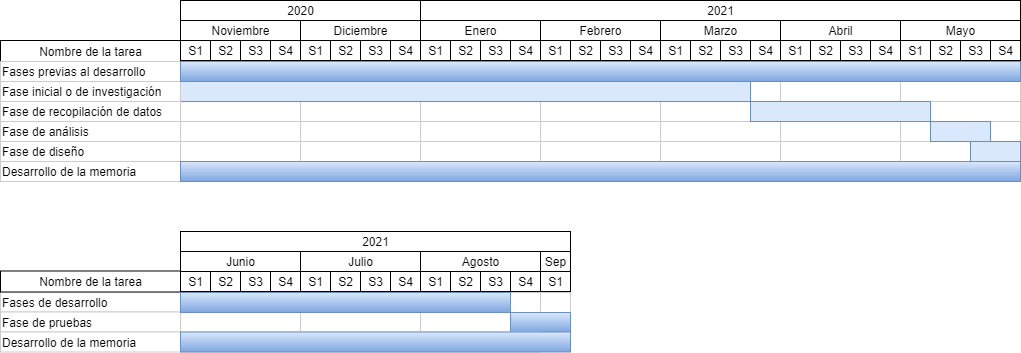
\includegraphics[width=1.2\textwidth]{imagenes/gantt.png}
	\caption{Diagrama de Gantt del proyecto}
\end{figure}




\section{Presupuesto}



